\documentclass{article}

\usepackage[english]{babel}
\usepackage[letterpaper,top=2cm,bottom=2cm,left=3cm,right=3cm,marginparwidth=1.75cm]{geometry}
\usepackage{amsmath}
\usepackage{amssymb}
\usepackage{amsthm}
\usepackage{comment}
\usepackage{enumitem}
\usepackage{graphicx}
\usepackage[colorlinks=true, allcolors=blue]{hyperref}
\usepackage[skip=20pt, indent=0pt]{parskip}
\usepackage{tikz}
    \usetikzlibrary{calc}
\usepackage{siunitx}
\usepackage{xcolor}

\title{Astrobiology 115 Homework 1}
\author{Alexandre Lipson}

\begin{document}
\maketitle


\section*{Chapter 1}

\begin{enumerate}

    \item
    \begin{figure*}[ht]
    \centering
    \begin{tikzpicture}
        \draw (0,0) ellipse (3cm and 2cm);
        % c^2 = a^2 - b^2 => c = sqrt(3^2-2^2) = sqrt(5) = ~2.236 
        \fill (-2.236,0) circle (2pt) node[above right] {Star Z};
        \fill (-3,0) circle (2pt) node[above left] {Planet A};
    \end{tikzpicture}
    \end{figure*}

    Use the diagram above to answer the following question. If planet A orbits star Z in 4 days (in a counterclockwise direction), 
    draw the position of planet A at day 1, day 2 and day 3. 
    (Hint: consider reviewing Kepler’s Laws) (3pts)

    \begin{figure*}[ht]
    \centering
    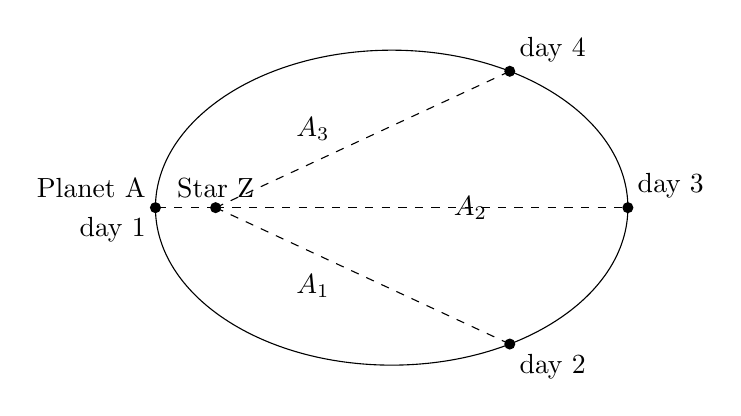
\begin{tikzpicture}
        \def\a{3}; % semimajor axis
        \def\b{2}; % semiminor axis
        
        \draw (0,0) ellipse ({\a} and {\b});
        

        \coordinate (focus) at ({-sqrt(\a^2-\b^2)},0);

        \coordinate (d1) at (-\a,0); % \coordinate (d1) at ({\a*cos(180)},{\b*sin(180)});
        \coordinate (d2) at ({\a*cos(-60)},{\b*sin(-60)});
        \coordinate (d3) at (\a,0);
        \coordinate (d4) at ({\a*cos(60)},{\b*sin(60)});

        \fill (focus) circle (2pt) node[above] {Star Z};
        \fill (d1) circle (2pt) node[below left] {day 1};
        \fill (d2) circle (2pt) node[below right] {day 2};
        \fill (d3) circle (2pt) node[above right] {day 3};
        \fill (d4) circle (2pt) node[above right] {day 4};

        \draw[dashed] (focus) -- (d1);
        \draw[dashed] (focus) -- (d2);
        \draw[dashed] (focus) -- (d3);
        \draw[dashed] (focus) -- (d4);

        \node[] at (-1, -1) {$A_1$};
        \node[] at (1, 0) {$A_2$};
        \node[] at (-1, 1) {$A_3$};

        \node[above left] at (d1) {Planet A};
    \end{tikzpicture}
    \end{figure*}

    By Kepler’s Second Law, $A_1=A_2=A_3$.

    \item People have long been interested in life beyond Earth. 
    What is different today that makes this possibility seem scientifically reasonable? (2pts)

    We are now able to understand how life formed on Earth, and how planets like Earth form in general. 
    We have discovered that organic compounds that are known to support life commonly form in the universe. This suggests that such molecules are present in many places. In addition, life started very early in Earth's history. Therefore, it is likely that the process to the inception of life is reasonably easy. Lastly, we have discovered life on our own planet that survives in a great variety of conditions. Examples of such organisms are extremophiles. All of these factors suggest that, with the many quadrillions of Earth-like planets in the universe, the possibility that two of them support life seems plausible.
    
    \item What are extrasolar planets? In what way does their discovery make it seem more reasonable to imagine finding life elsewhere? (2pts)
    
    Extrasolar planets, or exoplanets, are planets that belong to suns other than our own.
    We have found thousands of such planets, and some of which are at the right distance from their sun to allow for liquid water to persist.
    This adds to the number of places to look for life.

    Our current understanding of life is that it requires some solvent such as liquid water--ammonia or methane are other possibilities. Some planets may be host to such other forms of "life as we don't know it."

    \item What do we mean by a habitable planet? Does a habitable world necessarily have life? (1pts)
    
    Habitable planets are those that have the proper conditions for supporting life as we know it. 
    Our definition of habitable will change as we discover life that exists in new environments, such as extremophile microscopic organisms.
    
    A habitable world does not necessarily have life.
    
    \item What do we mean by the “universality” of physics and chemistry? 
    Although we don’t know yet whether biology is similarly universal, what evidence makes it seem that it might be? (2pts)
    
    Physics and chemistry are universal in that the laws that govern their functions on earth are the same laws that control physics and chemistry everywhere in our universe.
    In that sense, we expect that our understanding of biology, which is based on our understanding of both chemistry and physics, to also be universal everywhere.
    
    Furthermore, we have observed that organic molecules, which are necessary to our familiar carbon-based life, are quite prevalent in the universe. Therefore, for carbon life at least, the building blocks for living are available, so it would seem that the carbon-based biology as we understand it would be the most accessible path.

    \item Choose the best answer to each of the following. Explain your reasoning with one or more complete sentences. 
    By a geocentric view of the universe, we mean 
    \textcircled{a} the ancient idea that Earth resided at the center of the universe; 
    (b) the idea that Earth is the only planet with life in the universe; 
    (c) a view of the universe shaped by current understanding of geological science. (1pts)

    The word geocentric means, based on Greek roots, Earth at the center. Therefore, it's the idea that Earth is at the center of the universe.
    
    \item Choose the best answer to each of the following. Explain your reasoning with one or more complete sentences.
    According to current scientific understanding, life on Earth 
    (a) was exceedingly improbable; 
    \textcircled{b} arose quite soon after conditions allowed it;
    (c) may have been inevitable, but took billions of years to develop. (1pts)
    
    The earth formed about 4.6 billion years ago. The earliest evidence of life suggests that it may have begun about 3.7 billion years ago. This means that life began less than one billion years after the formation of the earth. This is a relatively short timeframe in the cosmic scale. 

    \item Choose the best answer to each of the following. Explain your reasoning with one or more complete sentences. 
    If we sent one of our current spacecraft to a nearby star (besides the Sun), the trip would take about 
    (a) a decade; 
    (b) a century; 
    \textcircled{c} 100,000 years. (1pts)

    The nearest star, proxima centauri is about 4.22 light years away.
    
    This distance is about, $4.22\si{ly}\frac{9.46 \cdot 10^{12} \si{km}}{1\si{ly}} = 3.99 \cdot 10^{13} \si{km}$.
    
    Our current spacecraft can travel at a top speed of $200 \si{\frac{km}{s}}$.

    Therefore the trip would take $3.99 \cdot 10^{13} \si{km} \left( \frac{1 \si{s}}{200 \si{km}} \right) = 2.00 \cdot 10^{11} \si{s}$.

    Converting seconds to years tells us that the trip would take about $2.00 \cdot 10^{11} \si{s} \left( \frac{}{} \right) = 6.34 \cdot 10^5 \si{years}$.

    This is on the same order of magnitude as option c, therefore about 100,000 years is closest estimate.
    
\end{enumerate}


\section{Chapter 2}

\begin{enumerate}[start=9]
    \item What is apparent retrograde motion, and why was it so difficult to explain with the geocentric model? What is its real explanation? (3pts)
    
    Apparent retrograde motion is when a star reverses the direction it travels in the night sky for a brief period. 
    It was difficult to explain with the geocentric model because, without the addition of complex subcircles, the only way for an object orbiting earth to go the other direction is for that object to actually go the other direction.
    The real explanation for apparent retrograde motion is that the planets orbit the sun and orbit at different speeds so there are positions where one planet is at the bottom of its orbit and another is just finishing the top, so the planet appears to be going the other direction with respect to the background of space.

    \item How did Newton’s discoveries about the laws of motion and the universal law of gravitation put the Sun-centered model on an even stronger footing? (1pts)

    Newton theorized that gravity is a force that originates from the inherit property of mass in objects. He claimed that more massive objects exert a greater gravitational pull. Therefore, since our
    Sun is much bigger and thus more massive than the Earth, it makes sense for the Earth to orbit it and not the other way around.

    \item Describe each of the three hallmarks of science and give an example of how we can see each one in the unfolding of the Copernican revolution. (6pts)
    
    \begin{enumerate}[label=\alph*.]
        \item Modern science seeks explanations for observations based only on natural phenomena. An example is when Kepler formulated an elliptical orbit hypothesis based upon Tycho Brahe's meticulous measurements of the stars.
        \item Science tests models and prefers those which explain everything as simple as possible, but no simpler. The latter principle is equivalent to Occam's philosophical razor. An example of this is when the Ptolemaic and Copernican models were tested against each other, while they both mode somewhat accurate predictions of the movement of the stars, the Copernican model--while not actually favored immediately at the time--was superior in that the heliocentric explanation was simpler--even though it required subcircles too--than the geocentric one.
        \item Scientific models make testable predictions which allow us to determine the accuracy of the model. One example of this aspect of science is with regard to the circular versus elliptical orbit models. The circular models that were comprised of many subcircles had impressive accuracy, but ultimately paled in comparison to the Keplerian elliptical orbits which provided much more accurate predictions that actually matched observations.
    \end{enumerate}

    
    \item Choose the best answer to each of the following. Explain your reasoning with one or more complete sentences. According to Kepler’s third law, 
    (a) Mercury travels fastest in the part of its orbit in which it is closest to the Sun; 
    \textcircled{b} Jupiter orbits the Sun at a faster speed than Saturn; 
    (c) all the planets have nearly circular orbits. (1pts)
    

    Kepler’s third law is that the square of an object's orbital period is proportional to the cube of its semimajor axis.
    This means that planets that have smaller semimajor axes, meaning that they orbit closer to the Sun, will have shorter orbital orbital periods. Therefore, since Jupiter is closer to the sun than Saturn, it must have a shorter orbital period.

    Even though it has a shorter orbital path distance, Kepler’s third law does not necessarily indicate that planets will orbit with faster speeds.

    Option a, that Mercury travels fastest at perihelion is a consequence of Kepler’s second law, not the third.

    Option c is not addressed by Kepler’s laws.

    Therefore, option b is the best choice; it is likely that Jupiter orbits the Sun at a faster speed than Saturn.
    
    More information would be needed, such as the mass of Jupiter and Saturn, to determine if Jupiter does indeed orbit faster.

    With regards to distance, we can research that both Jupiter and Saturn have eccentricities below 0.06. This means that their orbits are very circular. So, we can approximate their path length as the circumference of a circle such that the path length $l$, is defined by the semimajor axis $a$, $l \approx 2\pi a$ for low eccentricities.\footnote{Specifically, we can find the error of this estimate by taking the line integral of an ellipse with a set semimajor axis of 1 and varying the eccentricity. Eccentricity $e$ is defined as the ratio of the focus and the semimajor axis. We can define our ellipse by the equation $\frac{x^2}{a^2}+\frac{y^2}{b^2}=1$ where b is the semiminor axis. Then, with the relationship that the focus $c$ is defined by the ellipses axes $a$ and $b$, $c^2 = a^2 - b^2$, we can define the semiminor axis by the eccentricity of the ellipse, $b = \sqrt{a^2 - {(ae)}^2}$ We can simplify to $b = a\sqrt{1-e^2}$. We then parametrize the ellipse by trigonometric identities, \[\vec{r}(x(t),y(t)) = \left< a\cos{t}, b\sin{t} \right>.\] Then, we find the arc length of the path, where $2\pi$ is the period of the sine and cosine functions, \[\int_{0}^{2\pi} \sqrt{{(-a\sin{t})}^2 + {(b\cos{t})}^2} \ dt.\] This can be further simplified to, \[\int_{0}^{2\pi} a \sqrt{\sin^2{t} + (1-e^2)\cos^2{t}} \ dt.\] Noting that, with an eccentricity of zero, this reduces to $\int_{0}^{2\pi} a dt$, which we recognize to be the integral for the circumference of a circle with radius $a$. Therefore, we can evaluate the ratio between the arc length of an ellipse with eccentricity $e$ and the circumference of a circle to determine how the arc length decreases as eccentricity increases--where the radius is matched to the semimajor axis. We see that the, as the eccentricity approaches the maximum of 1, the arc length of an ellipse is a bit less than roughly 2/3 of the circumference of the circle with an equal semimajor axis.}
    We then take the ratio of the circle path distance and the period $T$ as a function of the semimajor axis $a$ from Kepler’s third law, $T^2 \propto a^3$, \[\frac{2\pi a}{ka^{\frac{3}{2}}} : k \in \mathbb{R}.\]
    So orbital speed, determined by the ratio of the orbit distance and orbit rate, is, \[\frac{2\pi}{k} a^{-\frac{1}{2}}.\]
    Since the speed increases as the semimajor axis increases and Jupiter is closer to the Sun than Saturn and both of their orbits are very circular, Jupiter orbits faster than Saturn.


    \item Choose the best answer to each of the following. Explain your reasoning with one or more complete sentences. Tycho Brahe’s contributions to astronomy included 
    (a) inventing the telescope; 
    (b) proving that Earth orbits the Sun; 
    \textcircled{c} collecting data that enabled Kepler to discover the laws of planetary motion. (1pts)
    
    Tycho Brahe used naked-eye astronomy to make his accurate observations. He did not invent the telescope.
    Copernicus was more responsible for demonstrating the heliocentric model.
    Therefore, option c is correct.

    \item Be sure to show all calculations clearly and state your final answers in complete sentences. 
    The object Sedna orbits our Sun at an average distance (semimajor axis) of 509 AU.
    What is its orbital period? (3pts)

    Based on Kepler’s third law, for orbital period $T$ and its semimajor axis $a$, $T^2 \propto a^3$. With distance in astronomical units and time in days, $\frac{a^3}{T^2} \approx \frac{GM}{4\pi^2}$, where $G$ is the gravitational constant, and $M$ is the mass of the sun. For our solar system, the constant $\frac{GM}{4\pi^2} \approx 7.5 \cdot 10^{-6} \frac{\si{AU}^3}{\si{days}^2}$.
    So, with $a = 509 \si{AU}$,
    \begin{align*}
        \frac{{(509 \si{ AU})}^3}{T^2} &\approx 7.5 \cdot 10^{-6} \frac{\si{ AU}^3}{\si{ days}^2} \\
        \frac{509^3}{7.5 \cdot 10^{-6}} \si{ days}^2 &\approx T^2 \\
        \sqrt{\frac{509^3}{7.5 \cdot 10^{-6}}} \si{ days} &\approx T \\
        4.2 \cdot 10^6 \si{ days} &\approx T \\
        4.2 \cdot 10^6 \si{ days} \frac{1 \si{ years}}{365.25 \si{ days}} &\approx T \\
        T &\approx 1.1 \cdot 10^4 \si{ years}.
    \end{align*}

    The orbital period of Sedna is about eleven thousand years.

\end{enumerate}


\section*{Chapter 3}

\begin{enumerate}[start=15]
    \item What do we mean when we say that the universe is expanding? How does expansion lead to the idea of the Big Bang? Briefly describe the evidence supporting the idea that our universe began with the Big Bang. (3pts)
    
    The space between structures in the universe is expanding. Specifically, by the Hubble constant, $H_0 \approx 70 \si{\frac{\frac{km}{s}}{Mpc}}$, which means that the universe is expanding by $70 \si{\frac{km}{s}}$ for every megaparsec of distance away from a given location.

    In addition to the expansion of the universe, there are several other observations that support the Big Bang Theory. 

    First, is the isotropic property of the universe. This means that, on the largest scales, structures look essentially homogenous in all directions.

    Second, is the cosmic microwave background radiation. This radiation fills space to provide mean temperature of about 2.7K. This suggests that the universe was once very small and very hot.

    Third, is the very high relative abundance of helium and hydrogen based on the nuclear synthesis that occurred in the early universe. As the universe begin to expand, the particles got farther away from each other and thus didn't undergo more nuclear fusion and therefore we are left with very atomically light particles in great abundance.

    \item Briefly describe the four major features of our solar system that provide clues to how it formed. (4pts)
    
    \begin{enumerate}
        \item The planets in the solar system orbit in more or less a single plane and in the same direction--although their orbital tilt does vary such that their rotational directions as viewed from above may not all be the same. This rotating plane is possible when angular momentum is conserved from a spinning spherical body of matter.
        
        \item The small terrestrial planets are at the inside of the solar system while the large icy and gaseous planets are on the outside of the solar system. This means that the heat from the sun prevented ice from forming inside of the snow line.
        
        \item There are also non-planetary objects such are the asteroid and Kuiper belts in addition to the Oort cloud which are comprised of the necessary components for planet formation such as dust and planetesimals.
        
        \item There are also some exceptions in our solar to the expected output of the nebular hypothesis. For example, the Earth is too massive and has too great of an iron content than would be predicted of a planet at its distance from the Sun. This is due largely to the influence of our Moon. Given this, we understand that solar system formation is unpredictable and influenced by random events.
    \end{enumerate}
    
    
    \item Choose the best answer to each of the following. Explain your reasoning with one or more complete sentences. According to observations, the overall chemical composition of our solar system and other similar star systems is approximately 
    \textcircled{a} 98\% hydrogen and helium, 2\% all other elements combined; 
    (b) 98\% ice, 2\% metal and rock; 
    (c) 100\% hydrogen and helium. (4pts)

    The solar system cannot be made of 100\% hydrogen and helium because I am currently alive and breathing oxygen on planet Earth. Therefore, since there is oxygen, the answer is not c.
    Likewise, I just drank some water. It was not ice, and its elements, oxygen and hydrogen are lighter than metal and rock--although, to astronomers, everything heavier than Helium is a metal. Therefore, b in not the correct choice either. 
    This leaves a, the correct choice.

    \item Choose the best answer to each of the following. Explain your reasoning with one or more complete sentences.
    The age of our solar system is about 
    \textcircled{a} one-third of the age of the universe; 
    (b) three-fourths of the age of the universe; 
    (c) 2 billion years less than the age of the universe. (1pts)

    Our solar system is thought to have formed about 4.6 billion years ago. The age of the universe is thought to be about 13.7 billion years old. Therefore, our solar system is about one-third of the age of the universe.
    
    \item Be sure to show all calculations clearly and state your final answers in complete sentences. Communication with Mars. 
    We use radio waves, which travel at the speed of light, to communicate with robotic spacecraft. 
    How long does it take a message to travel from Earth to a spacecraft on Mars when 
    (a) Mars is at its closest distance to Earth; 
    (b) Mars is at its farthest distance from Earth? 
    (Data: The distance from Earth to Mars ranges between about 56 and 400 million kilometers.) (5pts)

    The speed of light, $c$, is about $3.0 \cdot 10^5 \si{\frac{km}{s}}$.

    When Mars is closest to Earth,
    \[5.6 \cdot 10^7 \si{km} \cdot \frac{1 \si{s}}{3.0 \cdot 10^5 \si{km}} \cdot \frac{1 \si{min}}{60 \si{s}} \approx 3.1 \si{min}.\]

    When Mars is farthest from Earth,
    \[4.00 \cdot 10^8 \si{km} \cdot \frac{1 \si{s}}{3.0 \cdot 10^5 \si{km}} \cdot \frac{1 \si{min}}{60 \si{s}} \approx 22.2 \si{min}.\]

    Therefore, it takes about three minutes communicate with Mars when it is closest to earth and a bit more than 20 minutes to communicate when Mars is farthest away.

    \item Be sure to show all calculations clearly and state your final answers in complete sentences. Planet Probabilities. Suppose that only one in one million stars is orbited by an Earth-like planet. 
    If there are 100 billion stars in the Milky Way Galaxy, how many Earth-like planets are there in the galaxy? 
    If there are 100 billion galaxies in the observable universe, how many Earth-like planets are there in the observable universe? (3pts)
    
    First, with just the Milky Way galaxy:
    \[\frac{1 \text{ Earth-like planets}}{1 \cdot 10^6 \text{ Stars}} \cdot \frac{1 \cdot 10^{11} \text{ Stars}}{\text{Milky Way}} = \frac{1 \cdot 10^5 \text{ Earth-like planets}}{\text{Milky Way}}.\]
    So, we estimate that there are about one hundred thousand Earth-like planets in the Milky Way.

    Next, with the observable universe of Milky Way-like--with regards to proportion of Earth-like planets--galaxies.
    \[\frac{1 \cdot 10^5 \text{ Earth-like planets}}{1 \text{ Galaxies}} \cdot \frac{1 \cdot 10^{11} \text{ Galaxies}}{\text{Universe}} = \frac{1 \cdot 10^{16} \text{ Earth-like planets}}{\text{Universe}}.\]
    So, we predict that there are roughly ten quadrillion Earth-like planets in the universe.

\end{enumerate}


\end{document}